\section{Mô hình Camera Lỗ kim}
\label{sec:pinhole_camera_model}

Trong Thị giác Máy tính, một trong những câu hỏi cơ bản nhất là: làm thế nào thế giới ba chiều (3D) được biểu diễn thành một hình ảnh hai chiều (2D)? Để trả lời câu hỏi này, chúng ta cần một mô hình hình học mô tả quá trình tạo ảnh.

Mặc dù các camera hiện đại sử dụng hệ thống thấu kính phức tạp, phần lớn các thuật toán trong Thị giác Máy tính lại dựa trên một mô hình lý tưởng hóa đơn giản hơn rất nhiều: \textbf{mô hình camera lỗ kim (pinhole camera)}.

Mô hình này giả định rằng toàn bộ ánh sáng đi vào camera đều phải đi qua một điểm duy nhất trước khi chiếu lên mặt phẳng ảnh. Dù là một sự đơn giản hóa mạnh, mô hình này vẫn nắm bắt được bản chất hình học cốt lõi của quá trình tạo ảnh và là nền tảng cho hầu hết các hệ thống thị giác hiện đại.

\subsection{Nguyên lý Hình học Cơ bản}
\label{subsec:pinhole_geometry}

Hãy tưởng tượng một hộp kín hoàn toàn, với một lỗ nhỏ trên một mặt và một màn chiếu ở mặt đối diện. Ánh sáng từ môi trường bên ngoài đi qua lỗ này và tạo thành ảnh trên màn chiếu.

\begin{center}
	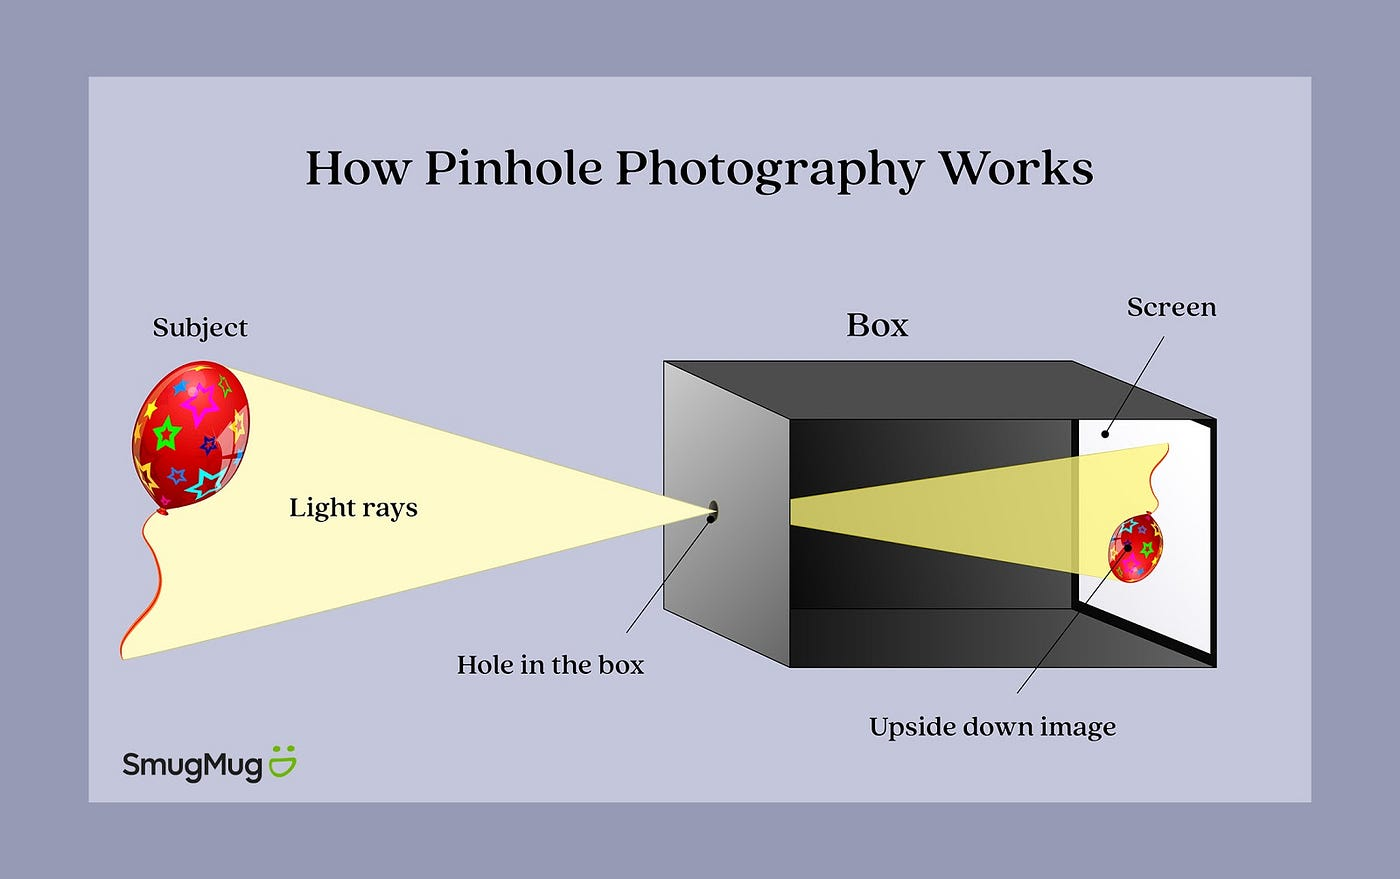
\includegraphics[width=0.75\textwidth]{images/pinhole_camera_basic.jpg}
	\captionof{figure}{Mô hình camera lỗ kim cơ bản. Ánh sáng từ các điểm trong không gian đi qua một điểm duy nhất (lỗ kim) trước khi tạo thành ảnh trên mặt phẳng.}
	\label{fig:pinhole_basic}
\end{center}

Một hiện tượng quan trọng xảy ra là: \textbf{ảnh bị lật ngược}. Điểm nằm phía trên trong thế giới sẽ xuất hiện phía dưới trên ảnh, và ngược lại.

Hiện tượng này xảy ra do các tia sáng từ các điểm khác nhau trong không gian giao nhau tại lỗ kim trước khi tiếp tục truyền đi. Sau khi giao nhau, chúng “đổi vị trí” tương đối trên mặt phẳng ảnh.

Trong thực tế, các camera sử dụng thấu kính để điều chỉnh hiện tượng này. Tuy nhiên, trong mô hình toán học, để tránh phải xử lý sự đảo ngược này, chúng ta sử dụng một khái niệm tiện lợi hơn.

\begin{mdframed}[style=infobox]
	\textbf{Quy ước mặt phẳng ảnh ảo (Virtual Image Plane)}
	
	Thay vì đặt mặt phẳng ảnh phía sau lỗ kim (như trong vật lý), chúng ta đặt nó phía trước lỗ kim, tại $Z = f$. Đây là một quy ước toán học giúp ảnh không bị lật ngược và đơn giản hóa các phép biến đổi.
	
	Lưu ý rằng đây không phải là vị trí vật lý thực của cảm biến, mà chỉ là một mô hình tương đương về mặt hình học.
\end{mdframed}

\subsection{Hệ Tọa độ Camera}
\label{subsec:pinhole_coordinate_system}

Để mô tả quá trình tạo ảnh một cách chính xác, chúng ta cần thiết lập một hệ tọa độ.

\begin{itemize}
	\item \textbf{Tâm camera (Camera center)}: Ký hiệu là $C$, đặt tại gốc tọa độ $(0,0,0)$
	\item \textbf{Trục quang học}: Trùng với trục $Z$
	\item \textbf{Mặt phẳng ảnh}: Đặt tại $Z = f$, với $f$ là tiêu cự
\end{itemize}

Một điểm trong không gian 3D (trong hệ tọa độ camera) được biểu diễn bởi:
\[
\mathbf{P}_c = (X, Y, Z)^T
\]

Mục tiêu của chúng ta là tìm ảnh của điểm này trên mặt phẳng ảnh:
\[
\mathbf{p} = (x, y)^T
\]

\subsection{Phép chiếu Phối cảnh}
\label{subsec:perspective_projection_derivation}

Mối quan hệ giữa điểm 3D và ảnh 2D của nó được xác định thông qua hình học tam giác đồng dạng.

\begin{center}
	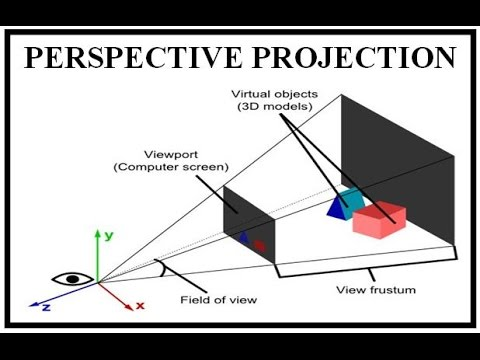
\includegraphics[width=0.75\textwidth]{images/perspective_projection.jpg}
	\captionof{figure}{Phép chiếu phối cảnh trong mô hình pinhole. Các tam giác đồng dạng tạo ra mối quan hệ giữa tọa độ 3D và 2D.}
	\label{fig:perspective_projection}
\end{center}

Từ hình học, ta có:

\[
\frac{x}{f} = \frac{X}{Z}, \quad \frac{y}{f} = \frac{Y}{Z}
\]

Suy ra:

\[
x = f \frac{X}{Z}, \quad y = f \frac{Y}{Z}
\]

Đây là \textbf{phép chiếu phối cảnh (perspective projection)}.

Công thức này cho thấy rõ bản chất của quá trình tạo ảnh: tọa độ ảnh phụ thuộc vào tỷ lệ giữa vị trí ngang/dọc và độ sâu.

\begin{mdframed}[style=infobox]
	\textbf{Hiệu ứng phối cảnh}
	
	Khi $Z$ tăng (vật ở xa hơn), các giá trị $\frac{X}{Z}$ và $\frac{Y}{Z}$ giảm, khiến điểm ảnh tiến gần về tâm ảnh. Điều này giải thích tại sao các vật thể ở xa trông nhỏ hơn và các đường song song dường như hội tụ về một điểm (vanishing point).
\end{mdframed}

\subsection{Tọa độ Thuần nhất và Biểu diễn Tuyến tính}
\label{subsec:homogeneous_coordinates_pinhole}

Phép chiếu phối cảnh là một phép biến đổi phi tuyến do có phép chia cho $Z$. Điều này gây khó khăn khi muốn biểu diễn bằng đại số tuyến tính.

Để giải quyết vấn đề này, chúng ta sử dụng \textbf{tọa độ thuần nhất (homogeneous coordinates)}.

Ta biểu diễn điểm ảnh dưới dạng:
\[
\mathbf{p} = (x, y, 1)^T
\]

Khi đó, phép chiếu có thể viết lại dưới dạng:

\[
s
\begin{bmatrix}
	x \\ y \\ 1
\end{bmatrix}
=
\begin{bmatrix}
	f & 0 & 0 \\
	0 & f & 0 \\
	0 & 0 & 1
\end{bmatrix}
\begin{bmatrix}
	X \\ Y \\ Z
\end{bmatrix}
\]

trong đó $s = Z$ là một hệ số tỷ lệ.

Ma trận:

\[
K =
\begin{bmatrix}
	f & 0 & 0 \\
	0 & f & 0 \\
	0 & 0 & 1
\end{bmatrix}
\]

được gọi là \textbf{ma trận nội tại (intrinsic matrix)} trong trường hợp đơn giản.

\begin{mdframed}[style=infobox]
	\textbf{Mô hình nội tại tổng quát}
	
	Trong thực tế, camera không lý tưởng. Ma trận nội tại đầy đủ có dạng:
	
	\[
	K =
	\begin{bmatrix}
		f_x & 0 & c_x \\
		0 & f_y & c_y \\
		0 & 0 & 1
	\end{bmatrix}
	\]
	
	trong đó $(c_x, c_y)$ là tâm ảnh (principal point), và $f_x, f_y$ có thể khác nhau do tỉ lệ pixel.
\end{mdframed}

\subsection{Từ Thế giới đến Ảnh}
\label{subsec:world_to_image}

Cho đến nay, chúng ta giả định điểm $\mathbf{P}_c$ đã được biểu diễn trong hệ tọa độ camera. Tuy nhiên, trong thực tế, các điểm thường được cho trong hệ tọa độ thế giới (world coordinates).

Do đó, chúng ta cần một phép biến đổi để chuyển từ hệ tọa độ thế giới sang hệ tọa độ camera:

\[
\mathbf{P}_c = R \mathbf{P}_w + t
\]

trong đó:
\begin{itemize}
	\item $R$: ma trận quay (rotation matrix)
	\item $t$: vector tịnh tiến (translation vector)
\end{itemize}

Kết hợp với phép chiếu, ta thu được mô hình tổng quát:

\[
s \mathbf{p} = K [R|t] \mathbf{P}_w
\]

Đây là phương trình cơ bản của camera trong Thị giác Máy tính, kết hợp cả:
\begin{itemize}
	\item \textbf{Extrinsic parameters}: $R, t$ (vị trí và hướng camera)
	\item \textbf{Intrinsic parameters}: $K$ (đặc tính nội tại của camera)
\end{itemize}

\subsection{Hạn chế của Mô hình}
\label{subsec:pinhole_limitations}

Mặc dù rất hữu ích, mô hình pinhole vẫn là một sự lý tưởng hóa:

\begin{itemize}
	\item Không xét đến biến dạng thấu kính (radial, tangential distortion)
	\item Giả định ánh sáng đi qua một điểm duy nhất
	\item Bỏ qua nhiễu, nhiễu xạ và các hiệu ứng vật lý khác
\end{itemize}

Tuy nhiên, trong nhiều bài toán, mô hình này là đủ chính xác và đóng vai trò nền tảng để xây dựng các mô hình phức tạp hơn.

\subsection*{Kết luận}
\label{subsec:pinhole_conclusion}

Mô hình camera lỗ kim cung cấp một khung toán học rõ ràng và mạnh mẽ để mô tả quá trình tạo ảnh. Từ một giả định đơn giản về cách ánh sáng truyền đi, chúng ta có thể xây dựng được một mô hình liên kết trực tiếp giữa thế giới 3D và ảnh 2D.

Quan trọng hơn, mô hình này không chỉ giải thích các hiện tượng trực quan như hiệu ứng phối cảnh, mà còn cho phép chúng ta biểu diễn toàn bộ quá trình bằng đại số tuyến tính. Đây chính là nền tảng cho hầu hết các thuật toán trong Thị giác Máy tính hiện đại.

Trong các phần tiếp theo, chúng ta sẽ tiếp tục mở rộng mô hình này để xử lý các tình huống thực tế phức tạp hơn, bao gồm hiệu chỉnh camera và tái tạo hình học 3D.

\section*{Tài liệu tham khảo}
\begin{itemize}
	\item[1] Hartley, R., \& Zisserman, A. (2003). \textit{Multiple View Geometry in Computer Vision}. Cambridge University Press.
	\item[2] Szeliski, R. (2010). \textit{Computer Vision: Algorithms and Applications}. Springer.
\end{itemize}